\let\lesson\undefined
\newcommand{\lesson}{\phantomlesson{Bài 8.}}
\section{Bài tập trắc nghiệm}
\begin{enumerate}[label=\bfseries Câu \arabic*:, leftmargin=1.7cm]
	\item\mkstar{1}\\
	Chọn phương án \textbf{sai}.\\
	Với một lượng khí lí tưởng không đổi, áp suất khí càng lớn khi
	\begin{mcq}(2)
		\item thể tích các phân tử khí càng nhỏ.
		\item nhiệt độ của khí càng lớn.
		\item thể tích bình chứa càng nhỏ.
		\item mật độ phân tử khí càng lớn.
	\end{mcq}
\hideall{
\textbf{Đáp án A.}
}

\item \mkstar{1}\\
Động năng chuyển động tịnh tiến trung bình của các phân tử khí phụ thuộc vào
\begin{mcq}(2)
	\item mật độ phân tử khí.
	\item khối lượng mole.
	\item áp suất khối khí.
	\item nhiệt độ khối khí.
\end{mcq}
\hideall{
\textbf{Đáp án D.}
}

\item \mkstar{2}\\
Trong quá trình đẳng nhiệt của một lượng khí lí tưởng nhất định, mật độ phân tử khí 
\begin{mcq}(2)
	\item tỉ lệ nghịch với áp suất.
	\item tỉ lệ thuận với áp suất.
	\item luôn không đổi.
	\item chưa đủ dữ kiện để kết luận.
\end{mcq}
\hideall{
\textbf{Đáp án B.}
}

\item \mkstar{2}\\
Khi một khối khí chứa trong bình kín được cung cấp nhiệt, điều nhận định nào sau đây là \textbf{đúng}?
\begin{mcq}(2)
	\item áp suất khí giảm.
	\item thế năng của khối khí tăng.
	\item động năng của các phân tử khí tăng.
	\item thế năng của khối khí giảm.
\end{mcq}
\hideall{
\textbf{Đáp án C.}
}

\item \mkstar{2}\\
Điều nào sau đây là \text{đúng} khi nói về nội năng của khí lí tưởng?
\begin{mcq}(2)
	\item Chỉ phụ thuộc vào nhiệt độ của khối khí.
	\item Bằng tổng thế năng tương tác giữa các phân tử.
	\item Phụ thuộc vào thể tích khối khí.
	\item Không phụ thuộc vào số phân tử khí.
\end{mcq}
\hideall{
\textbf{Đáp án A.}
}

\item \mkstar{2}\\
Trong quá trình biến đổi đẳng nhiệt của một khối khí lí tưởng thì
\begin{mcq}(2)
	\item nội năng khí tăng.
	\item nội năng khí giảm.
	\item khí không thực hiện công.
	\item không có sự biến thiên nội năng.
\end{mcq}
\hideall{
\textbf{Đáp án D.}
}

\item\mkstar{2}\\
Trong quá trình biến đổi đẳng nhiệt của một khối khí lí tưởng thì toàn bộ nhiệt lượng mà khí nhận được 
\begin{mcq}
	\item chuyển hết thành công mà khí sinh ra.
	\item chuyển hết thành nội năng của khí.
	\item một phần làm tăng nội năng và phần còn lại biến thành công mà khí sinh ra.
	\item truyền nhiệt hết cho ngoại vi.
\end{mcq}
\hideall{
\textbf{Đáp án A.}
}

\item \mkstar{2}\\
Hệ thức nào sau đây phù hợp với quá trình đun nóng đẳng tích?
\begin{mcq}(2)
	\item $\Delta U=Q+A$ với $Q,A>0$.
	\item $\Delta U=Q$ với $Q>0$.
	\item $\Delta U=Q+A$ với $A<0$ và $Q>0$.
	\item $Q+A=0$.
\end{mcq}
\hideall{
\textbf{Đáp án B.}
}

\item \mkstar{2}\\
Hệ thức nào sau đây phù hợp với quá trình nén khí đẳng nhiệt?
\begin{mcq}(2)
	\item $Q+A=0$ với $A<0$.
	\item $\Delta U=Q+A$ với $\Delta U>0$, $Q<0$, $A>0$.
	\item $Q+A=0$ với $A>0$.
	\item $\Delta U=Q+A$ với $\Delta U>0$, $A>0$, $Q>0$.
\end{mcq}
\hideall{
\textbf{Đáp án C.}
}

\item \mkstar{2}\\
Trong quá trình đẳng tích, toàn bộ nhiệt lượng mà khí nhận được
\begin{mcq}
	\item chuyển hết thành công mà khí sinh ra.
	\item chuyển hết thành nội năng của khí.
	\item một phần làm tăng nội năng và phần còn lại biến thành công mà khí sinh ra.
	\item truyền nhiệt hết cho ngoại vi.
\end{mcq}
\hideall{
\textbf{Đáp án B.}
}

\item \mkstar{2}\\
Hệ thức nào sau đây phù hợp với quá trình làm lạnh đẳng tích?
\begin{mcq}(2)
	\item $\Delta U=A$ với $A>0$.
	\item $\Delta U=A$ với $A<0$.
	\item $\Delta U=Q$ với $Q>0$.
	\item $\Delta U=Q$ với $Q<0$.
\end{mcq}
\hideall{
\textbf{Đáp án D.}
}

\item \mkstar{2}\\
Trong quá trình đẳng áp, toàn bộ nhiệt lượng mà khí nhận được
\begin{mcq}
	\item chuyển hết thành công mà khí sinh ra.
	\item chuyển hết thành nội năng của khí.
	\item một phần làm tăng nội năng và phần còn lại biến thành công mà khí sinh ra.
	\item truyền nhiệt hết cho ngoại vi.
\end{mcq}
\hideall{
	\textbf{Đáp án C.}
}


\item \mkstar{3}\\
Khối lượng riêng của một chất khí bằng $\SI{6E-2}{\kilogram/\meter^3}$, tốc độ căn quân phương của các phân tử khí là $\SI{500}{\meter/\second}$. Áp suất mà khí đó tác dụng lên thành bình là
\begin{mcq}(4)
	\item $\SI{10}{\pascal}$.
	\item $\SI{E4}{\pascal}$.
	\item $\SI{5e3}{\pascal}$.
	\item $\SI{5E4}{\pascal}$.
\end{mcq}
\hideall{
\textbf{Đáp án C.}\\
$$p=\dfrac{1}{3}\rho \overline{v^2}=\SI{5E3}{\pascal}.$$
}

\item \mkstar{3}\\
Khối lượng riêng của một chất khí ở áp suất $\SI{300}{\milli\meter Hg}$ là $\SI{0.3}{\kilogram/\meter^3}$. Tốc độ căn quân phương của các phân tử khí khi đó gần bằng
\begin{mcq}(4)
	\item $\SI{3000}{\meter/\second}$.
	\item $\SI{630}{\meter/\second}$.
	\item $\SI{55}{\meter/\second}$.
	\item $\SI{500}{\meter/\second}$.
\end{mcq}
\hideall{
\textbf{Đáp án B.}\\
$$p=\dfrac{1}{3}\rho \overline{v^2}\Rightarrow \sqrt{\overline{v^2}}\approx\SI{630}{\meter/\second}.$$
}

\item \mkstar{3}\\
Số phân tử khí hydrogen chứa trong $\SI{1}{\meter^3}$ có áp suất $\SI{200}{\milli\meter Hg}$ và tốc độ căn quân phương $\SI{2400}{\meter/\second}$ là
\begin{mcq}(4)
	\item $\SI{4E24}{\text{phân tử}}$.
	\item $\SI{4E21}{\text{phân tử}}$.
	\item $\SI{E28}{\text{phân tử}}$.
	\item $\SI{E25}{\text{phân tử}}$.
\end{mcq}
\hideall{
\textbf{Đáp án A.}\\
$$p=\dfrac{1}{3}\cdot\dfrac{N}{V}\cdot\dfrac{\mu}{N_A}\cdot\overline{v^2}\Rightarrow N=\dfrac{3pVN_A}{\mu \overline{v^2}}=\SI{4E24}{}.$$
}

\item \mkstar{3}\\
Động năng chuyển động nhiệt trung bình của phân tử khí lí tưởng đơn nguyên tử ở nhiệt độ $\SI{27}{\celsius}$ là
\begin{mcq}(4)
	\item $\SI{3.3E-22}{\joule}$.
	\item $\SI{1.1E-21}{\joule}$.
	\item $\SI{2.76E-21}{\joule}$.
	\item $\SI{6.2E-21}{\joule}$.
\end{mcq}
\hideall{
\textbf{Đáp án D.}\\
$$W_\text{đ}=\dfrac{3}{2}kT\approx\SI{6.2E-21}{\joule}.$$
}

\item \mkstar{3}\\
Biết khối lượng mol của không khí là $\SI{29}{\gram/\mole}$. Tốc độ căn quân phương của các phân tử không khí ở nhiệt độ $\SI{17}{\celsius}$ là
\begin{mcq}(4)
	\item $\SI{15.6}{\meter/\second}$.
	\item $\SI{500}{\meter/\second}$.
	\item $\SI{243}{\meter/\second}$.
	\item $\SI{2.5}{\kilo\meter/\second}$.
\end{mcq}
\hideall{
\textbf{Đáp án B.}\\
$$\sqrt{\overline{v^2}}=\sqrt{\dfrac{3RT}{\mu}}\approx\SI{500}{\meter/\second}.$$
}

\item \mkstar{3}\\
Tổng động năng trung bình của $\SI{1}{\kilogram}$ khí helium ở nhiệt độ $\SI{1000}{\kelvin}$ là
\begin{mcq}(4)
	\item $\SI{5}{\mega\joule}$.
	\item $\SI{5}{\kilo\joule}$.
	\item $\SI{3}{\mega\joule}$.
	\item $\SI{3}{\kilo\joule}$.
\end{mcq}
\hideall{
\textbf{Đáp án C.}\\
$$U=\dfrac{3}{2}\cdot\dfrac{m}{\mu} RT=\SI{3}{\mega\joule}.$$
}

\item \mkstar{3}\\
Khí lí tưởng đơn nguyên tử trong bình kín $\SI{2}{\liter}$ có nội năng $\SI{300}{\joule}$ thì áp suất của khí là 
\begin{mcq}(4)
	\item $\SI{E5}{\newton/\meter^2}$.
	\item $\SI{E4}{\newton/\meter^2}$.
	\item $\SI{700}{\milli\meter Hg}$.
	\item $\SI{2.25E5}{\newton/\meter^2}$.
\end{mcq}
\hideall{
\textbf{Đáp án A.}\\
$$U=\dfrac{3}{2}\nu RT=\dfrac{3}{2}pV\Rightarrow p=\dfrac{2U}{3V}=\SI{E5}{\newton/\meter^2}.$$
}

\item \mkstar{3}\\
Người ta thực hiện công $A=\SI{124.65}{\joule}$ lên $\SI{2}{\mole}$ khí lí tưởng đơn nguyên tử thì nhiệt độ khối khí tăng thêm bao nhiêu? Biết rằng trong quá trình đó không có sự truyền nhiệt.
\begin{mcq}(4)
	\item $\SI{10}{\kelvin}$.
	\item $\SI{8}{\kelvin}$.
	\item $\SI{4}{\kelvin}$.
	\item $\SI{5}{\kelvin}$.
\end{mcq}
\hideall{
\textbf{Đáp án D.}\\
$$\Delta U=A=\dfrac{3}{2}\nu RT\Rightarrow \Delta T\approx\SI{5}{\kelvin}.$$
}

\item \mkstar{3}\\
Làm biến đổi một lượng khí từ trạng thái 1 sang trạng thái 2, biết rằng ở trạng thái 2 của áp suất và thể tích của khí đều lớn hơn trạng thái 1. Trong những cách làm biến đổi lượng khí sau đây, cách nào lượng khí sinh công nhiều nhất?
\begin{mcq}
	\item Đun nóng khí đẳng tích rồi đun nóng đẳng áp.
	\item Đun nóng khí đẳng áp rồi đun nóng đẳng tích.
	\item Đun nóng khí sao cho cả thể tích và áp suất của khí đều tăng tuyến tính và liên tục từ trạng thái 1 đến trạng thái 2.
	\item Đun nóng khí sao cho cả thể tích và áp suất khí đều tăng không tuyến tính và liên tục từ trạng thái 1 đến trạng thái 2.
\end{mcq}
\hideall{
\textbf{Đáp án A.}
}

\item \mkstar{3}\\
Piston được đẩy từ vị trí A đến vị trí B để nén khí trong đó bằng hai cách:
\begin{center}
	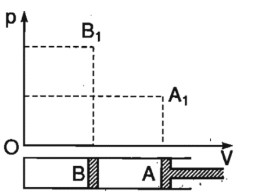
\includegraphics[width=0.35\linewidth]{../figs/VN12-Y24-PH-SYL-015P-3}
\end{center}
\begin{enumerate}[label=(\arabic*)]
	\item Đẩy rất chậm từ A đến B.
	\item Đẩy rất nhanh từ A đến B rồi chờ cho trạng thái khí ổn định.
\end{enumerate}
Cho biết công nén trong quá trình nào lớn hơn?
\begin{mcq}(2)
	\item Cách 1.
	\item Cách 2.
	\item Hai cách như nhau.
	\item Không thể kết luận được.
\end{mcq}
\hideall{
\textbf{Đáp án B.}\\
\begin{itemize}
	\item \textbf{Cách 1:} Do nén chậm nên nhiệt độ khí không đổi. Lúc này công khí nhận bằng độ biến thiên nội năng:
	$$A_1=\Delta U.$$
	\item \textbf{Cách 2:} Nén nhanh khi nên nhiệt độ khí tăng nhanh (do không kịp toả nhiệt) nên công khí nhận vừa làm tăng nội năng khí vừa làm cho khí nóng lên.
	$$A_2=\Delta U+Q.$$
\end{itemize}
}

\item \mkstar{3}\\
Độ biến thiên nội năng của khối khí lí tưởng đơn nguyên tử từ trạng thái $V_1=\SI{10}{\liter}$ và $p_1=\SI{1.5E5}{\pascal}$ đến trạng thái $V_2=\SI{20}{\liter}$ và $p_2=\SI{0.5E5}{\pascal}$ là
\begin{mcq}(4)
	\item $\Delta U=\SI{1150}{\joule}$.
	\item $\Delta U=\SI{-750}{\joule}$.
	\item $\Delta U=\SI{-1150}{\joule}$.
	\item $\Delta U=\SI{750}{\joule}$.
\end{mcq}
\hideall{
\textbf{Đáp án B.}\\
$$\Delta U=\dfrac{3}{2}\nu R\left(T_2-T_1\right)=\dfrac{3}{2}\left(p_2V_2-p_1V_1\right)=\SI{-750}{\joule}.$$
}

\item \mkstar{3}\\
Một cylanh thẳng đứng tiết diện $\SI{100}{\centi\meter^2}$ chứa khí ở nhiệt độ $\SI{27}{\celsius}$, phía trên được đậy bằng piston kín và cách nhiệt. Piston nhẹ, phía trên có đặt một vật nặng khối lượng $\SI{100}{\kilogram}$ và ban đầu cách đáy $\SI{60}{\centi\meter}$. Đốt nóng cylanh một cách từ từ để nhiệt độ khí tăng thêm $\SI{50}{\celsius}$. Cho áp suất khí quyển là $\SI{1.01E5}{\pascal}$, $g=\SI{9.8}{\meter/\second^2}$. Công do khí thực hiện là 
\begin{mcq}(4)
	\item $\SI{102}{\joule}$.
	\item $\SI{199}{\joule}$.
	\item $\SI{1200}{\joule}$.
	\item $\SI{98}{\joule}$.
\end{mcq}
\hideall{
\textbf{Đáp án B.}\\
Áp suất khí bên trong cylanh:
$$p=p_0+\dfrac{mg}{S}=\SI{199E3}{\pascal}.$$
Thể tích ban đầu của khí:
$$V_1=Sh_1=\SI{6E3}{\centi\meter^3}.$$
Đun từ từ nên áp suất khí trong cylanh không thay đổi:
$$\dfrac{V_1}{T_1}=\dfrac{V_2}{T_2}\Rightarrow V_2=\SI{7E3}{\centi\meter^3}.$$
Công do khí thực hiện:
$$A'=p\left(V_2-V_1\right)=\SI{199}{\joule}.$$
}

\item \mkstar{4}\\
Cho $\SI{1}{\mole}$ khí lí tưởng, khí thực hiện chu trình biến đổi trạng thái  $1-2-3-4-1$ như đồ thị trong hệ toạ độ $OVp$ ở hình bên. Các trạng thái 1 và 3 nằm trên cùng đường đẳng nhiệt. Nhiệt độ trạng thái 4 là $T_4=\SI{300}{\kelvin}$ và nhiệt độ ở trạng thái 2 là $T_2=\SI{390}{\kelvin}$. Công của khí nhận trên cả chu trình \textbf{gần nhất} với giá trị nào sau đây?
\begin{center}
	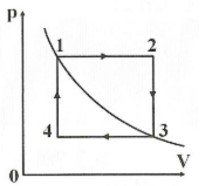
\includegraphics[width=0.3\linewidth]{../figs/VN12-Y24-PH-SYL-015P-5}
\end{center}
\begin{mcq}(4)
	\item $\SI{50}{\joule}$.
	\item $\SI{60}{\joule}$.
	\item $\SI{70}{\joule}$.
	\item $\SI{30}{\joule}$.
\end{mcq}
\hideall{
\textbf{Đáp án A.}\\
\begin{center}
	\begin{tabular}{|C{3cm}|C{3cm}|C{3cm}|C{3cm}|}
		\hline
		\thead{Trạng thái} & $p$ & $V$ & $T$\\
		\hline
		1 & $p_1$ & $V_1$ & $T$\\
		\hline
		2 & $p_1$ & $V_3$ & $\SI{390}{\kelvin}$\\
		\hline
		3 & $p_3$ & $V_3$ & $T$\\
		\hline
		4 & $p_3$ & $V_1$ & $\SI{300}{\kelvin}$\\
		\hline
	\end{tabular}
\end{center}
$$\dfrac{pV}{T}=\text{const}\Rightarrow \dfrac{p_1V_1}{T_1}=\dfrac{p_1V_3}{390}=\dfrac{p_3V_3}{T}=\dfrac{p_3V_1}{300}=R\Rightarrow \begin{cases}
	p_1V_3=390R\\
	p_1V_1=p_3V_3=RT\\
	p_3V_1=300R
\end{cases}\Rightarrow T=\sqrt{390\cdot300}=\xsi{30\sqrt{130}}{\kelvin}.$$
Công của chu trình:
$$A=\left(p_1-p_3\right)\left(V_3-V_1\right)=p_1V_3-p_1V_1-p_3V_3+p_3V_1=\left(390-30\sqrt{130}-30\sqrt{130}+300\right)R\approx\SI{49}{\joule}.$$
}
\end{enumerate}

\section{Trắc nghiệm đúng/sai}
\begin{enumerate}[label=\bfseries Câu \arabic*:, leftmargin=1.7cm]
	\item\mkstar{2}\\
	Một khối khí có thể tích $V_1=\SI{4}{\liter}$, áp suất $p=\SI{2E5}{\pascal}$ và nhiệt độ $t_1=\SI{57}{\celsius}$. Người ta thực hiện công $\SI{40}{\joule}$ để nén đẳng áp khối khí.
	\begin{enumerate}[label=\alph*)]
		\item Đồ thị biểu diễn quá trình nén khí trong hệ toạ độ $OpV$ là đoạn thẳng song song trục $OV$.
		\item Thể tích của khí sau khi nén bằng $\SI{3.8}{\liter}$.
		\item Nhiệt độ của khối khí sau khi nén bằng $\SI{313.5}{\celsius}$.
		\item Trong quá trình nén khí, khí toả nhiệt cho ngoại vi.
	\end{enumerate}
\hideall{
	\begin{enumerate}[label=\alph*)]
		\item Đúng.
		\item Đúng.
		$$A'=p\left(V_2-V_1\right)=\SI{-40}{\joule}\Rightarrow V_2=\SI{3.8E-3}{\meter^3}.$$
		\item Sai.\\
		$$\dfrac{V_1}{T_1}=\dfrac{V_2}{T_2}\Rightarrow T_2=\SI{313.5}{\kelvin}.$$
		\item Đúng. Vì $\Delta T<0$.
	\end{enumerate}

}


\item \mkstar{3}\\
Một khối khí lí tưởng có áp suất $p_1=\SI{3E3}{\pascal}$, thể tích $V_1=\SI{5}{\liter}$, nhiệt độ $t_1=\SI{27}{\celsius}$ được đun nóng đẳng áp đến nhiệt độ $t_2=\SI{177}{\celsius}$.
\begin{enumerate}[label=\alph*)]
	\item Trong quá trình đun, khối khí thực hiện công.
	\item Thể tích lúc sau của khối khí là $\SI{32.7}{\liter}$.
	\item Công mà khối khí thực hiện có độ lớn bằng $\SI{7.5}{\joule}$.
	\item Nếu nhiệt lượng mà khí nhận được là $\SI{18.75}{\joule}$ thì độ biến thiên nội năng của khí là $\SI{26.25}{\joule}$. 
\end{enumerate}
\hideall{
\begin{enumerate}[label=\alph*)]
	\item Đúng.
	\item Sai.
	$$\dfrac{V_1}{T_1}=\dfrac{V_2}{T_2}\Rightarrow V_2=\SI{7.5}{\liter}.$$
	\item Đúng.
	$$A'=p\left(V_2-V_1\right)=\SI{7.5}{\joule}.$$
	\item Sai.
	$$\Delta U=Q+A=\SI{18.75}{\joule}-\SI{7.5}{\joule}=\SI{11.25}{\joule}.$$
\end{enumerate}
}

\item \mkstar{3}\\
Một chiếc xe vượt qua sa mạc Sahara. Chuyến đi bắt đầu vào sáng sớm khi nhiệt độ là $\SI{3.0}{\celsius}$. Thể tích khí chứa trong mỗi lốp xe là $\SI{1.5}{\meter^3}$ và áp suất trong các lốp xe là $\SI{3.42E5}{\pascal}$. Coi khí trong lớp xe có nhiệt độ bằng nhiệt độ ngoài trời, không thoát ra ngoài và thể tích lốp không thay đổi. Đến giữa trưa, nhiệt độ tăng lên đến $\SI{42}{\celsius}$.
\begin{center}
	
\includegraphics[width=0.35\linewidth]{../figs/VN12-Y24-PH-SYL-015P-2}
\end{center}
\begin{enumerate}[label=\alph*)]
	\item  Trong mỗi lốp xe có $\SI{164}{\mole}$ khí.
	\item Tốc độ căn quân phương của khí bên trong lốp xe vào giữa trưa tăng lên 1,07 lần so với lúc sáng sớm.
	\item Khi đến giữa trưa, áp suất khí trong lốp xe là $\SI{3.9E5}{\pascal}$.
	\item Từ sáng đến giữa trưa, động năng tịnh tiến trung bình của một phân tử khí trong lốp xe tăng $\SI{9.5E-21}{\joule}$.
\end{enumerate}
\hideall{
\begin{enumerate}[label=\alph*)]
	\item  Sai.\\
	$$\nu=\dfrac{p_1V_1}{RT_1}\approx\SI{224}{\mole}.$$
	\item Đúng.
	$$\sqrt{\overline{v^2}}=\sqrt{\dfrac{3RT}{\mu}}\Rightarrow \dfrac{\sqrt{\overline{v^2_2}}}{\overline{v^2_1}}=\sqrt{\dfrac{T_2}{T_1}}=1,07.$$
	\item Đúng.
	$$\dfrac{p_2}{T_2}=\dfrac{p_1}{T_1}\Rightarrow p_2\approx\SI{3.9E5}{\pascal}.$$
	\item Sai.\\
	$$\Delta W_\text{đ}=\dfrac{3}{2}k\Delta T\approx\SI{8E-22}{\joule}.$$
\end{enumerate}
}

\item \mkstar{3}\\
Khí helium đựng trong bình kín có thể tích $\SI{2}{\liter}$ ở nhiệt độ $\SI{27}{\celsius}$, áp suất $\SI{E5}{\pascal}$. Sau đó, người ta đung nóng khí trong bình đến nhiệt độ $\SI{127}{\celsius}$.
\begin{enumerate}[label=\alph*)]
	\item Khối lượng riêng của khí helium ở nhiệt độ $\SI{27}{\celsius}$ là $\SI{160}{\kilogram/\meter^3}$.
	\item Tốc độ căn quân phương của mỗi nguyên tử khí ở trạng thái ban đầu là $\SI{1579}{\meter/\second}$.
	\item Trong quá trình đun nóng, khí không thực hiện công.
	\item Nhiệt lượng cung cấp để đun nóng khí trong điều kiện nói trên là $\SI{100}{\joule}$.
\end{enumerate}
\hideall{
\begin{enumerate}[label=\alph*)]
	\item Sai.
	$$\rho=\dfrac{p\mu}{RT}\approx\SI{0.16}{\kilogram/\meter^3}.$$
	\item Sai.
	$$\sqrt{\overline{v^2_1}}=\sqrt{\dfrac{3RT_1}{\mu}}\approx\SI{1368}{\meter/\second}.$$
	\item Đúng.
	\item Đúng. Vì $A=0$ nên
	$$Q=\Delta U=\dfrac{3}{2}\nu R\left(T_2-T_1\right)=\dfrac{3}{2}\cdot\dfrac{p_1V_1}{T_1}\cdot\left(T_2-T_1\right)=\SI{100}{\joule}.$$
\end{enumerate}
}

\item \mkstar{3}\\
Một khối khí helium chứa trong bình có thể tích $\SI{5}{\liter}$, áp suất $\SI{1.5E5}{\newton/\meter^2}$. Nén đẳng áp khối khí để mật độ phân tử tăng gấp hai lần.
\begin{enumerate}[label=\alph*)]
	\item Động năng trung bình của phân tử khí trước khi nén là $\SI{6.2E-11}{\joule}$.
	\item Mật độ phân tử khí trước khi nén là $\SI{3.6E-25}{\meter^{-3}}$.
	\item Nhiệt độ của khí sau khi nén là $\SI{150}{\celsius}$.
	\item Nhiệt lượng khí truyền cho bên ngoài là $\SI{562.5}{\joule}$.
\end{enumerate}
\hideall{
\begin{enumerate}[label=\alph*)]
	\item Đúng.
	$$W_\text{đ}=\dfrac{3}{2}kT\approx\SI{6.2E-21}{\joule}.$$
	\item Đúng.
	$$n=\dfrac{N}{V}=\dfrac{p}{kT}\approx\SI{3.6E25}{\meter^{-3}}.$$
	\item Sai.
	$$\dfrac{n_2}{n_1}=\dfrac{T_1}{T_2}\Rightarrow T_2=\SI{150}{\kelvin}\rightarrow t_2=\SI{-123}{\celsius}.$$
	\item Sai.
	$$Q=\Delta U+A'=\dfrac{3}{2}\nu R\left(T_2-T_1\right)+p\left(V_2-V_1\right)=\dfrac{5}{2}p\left(V_2-V_1\right)=\SI{-937.5}{\joule}.$$
\end{enumerate}
}
	
\end{enumerate}
\section{Bài tập tự luận}
\begin{enumerate}[label=\bfseries Câu \arabic*:, leftmargin=1.7cm]
	\item\mkstar{3}\\
	Ở nhiệt độ phòng và áp suất $\SI{E5}{\pascal}$, không khí có khối lượng riêng khoảng $\SI{1.29}{\kilogram/\meter^3}$. Xác định giá trị trung bình của bình phương tốc độ các phân tử khí.
	\hideall{
$$p=\dfrac{1}{3}\rho \overline{v^2}\Rightarrow \overline{v^2}\approx\SI{23E4}{\meter^2/\second^2}.$$	
}

\item \mkstar{3}\\
Để động năng tịnh tiến trung bình của các phân tử khí bằng $\SI{1.0}{\electronvolt}$ thì nhiệt độ của khối khí phải bằng bao nhiêu $\si{\kelvin}$? Lấy $\SI{1}{\electronvolt}=\SI{1.6E-19}{\joule}$.
\hideall{
$$W_\text{đ}=\dfrac{3}{2}kT\Rightarrow T\approx\SI{7729}{\kelvin}.$$
}

\item \mkstar{3}\\
Một bình dung tích $\SI{7.5}{\liter}$ chứa $\SI{24}{\gram}$ khí oxygen ở áp suất $\SI{2.5E5}{\newton/\meter^2}$. Tính động năng tịnh tiến trung bình của mỗi phân tử khí oxygen.
\hideall{
$$W_\text{đ}=\dfrac{3}{2}kT=\dfrac{3}{2}\cdot\dfrac{RT}{N_A}=\dfrac{3}{2}\cdot\dfrac{M pV}{mN_A}\approx\SI{6.23E-21}{\joule}.$$
}

\item \mkstar{3}\\
Tính trung bình của bình phương tốc độ trong chuyển động nhiệt của phân tử khí helium có khối lượng mol là $\SI{4}{\gram/\mole}$ ở nhiệt độ $\SI{320}{\kelvin}$.
\hideall{
$$W_\text{đ}=\dfrac{1}{2}m\overline{v^2}=\dfrac{3}{2}\cdot\dfrac{RT}{N_A}\Leftrightarrow \dfrac{1}{2}\cdot\dfrac{M}{N_A}\cdot\overline{v^2}=\dfrac{3}{2}\cdot\dfrac{RT}{N_A}\Rightarrow \overline{v^2}=\dfrac{3RT}{M}\approx\SI{2E6}{\meter^2/\second^2}.$$
}

\item \mkstar{3}\\
Xét khối khí trong bình kín, biết mật độ động năng phân tử (tổng động năng tịnh tiến trung bình của các phân tử khí trong $\SI{1}{\meter^3}$ khí) có giá trị $\SI{E-4}{\joule/\meter^3}$. Tính áp suất khí trong bình.
\hideall{
$$\omega_\text{đ}=\dfrac{\sum W_\text{đ}}{V}=\dfrac{3}{2}\cdot\dfrac{n RT}{V}=\dfrac{3}{2}p\Rightarrow p=\dfrac{2}{3}\omega_\text{đ}\approx\SI{6.67E-5}{\pascal}.$$
}

\item \mkstar{3}\\
Bình thể tích $\SI{10}{\liter}$ chứa khí đơn nguyên tử có mật độ $\mu=\SI{3E-24}{\meter^{-3}}$. Động năng trung bình của nguyên tử là $\SI{5E-21}{\joule}$. Nội năng của khí trong bình bằng bao nhiêu?
\hideall{
$$\mu=\dfrac{N}{V}\Rightarrow N=\mu V.$$
Nội năng của khí:
$$U=NW_\text{đ}=\mu V W_\text{đ}=\SI{150}{\joule}.$$
}

\item \mkstar{3}\\
Cho $\SI{20}{\gram}$ khí oxygen ở áp suất $\SI{2E5}{\newton/\meter^2}$, nhiệt độ $\SI{31}{\celsius}$ được đun nóng đẳng áp và dãn nở đến thể tích $\SI{25}{\liter}$. Công mà khí thực hiện trong quá trình trên bằng bao nhiêu?
\hideall{
$$p_1V_1=\dfrac{m}{M}RT_1\Rightarrow V_1\approx\SI{7.9E-3}{\meter^3}.$$
Công khí thực hiện:
$$A'=p\left(V_2-V_1\right)\approx\SI{3.4}{\kilo\joule}.$$
}

\item \mkstar{3}\\
Cho $\SI{12}{\gram}$ khí hydrogen dãn nở đẳng áp, thể tích tăng gấp ba lần và thực hiện công $\SI{29916}{\joule}$. Nhiệt độ ban đầu của khí bằng bao nhiêu?
\hideall{
Số mol khí:
$$n=\dfrac{m}{M}=\SI{6}{\mole}.$$
Qúa trình đẳng áp:
$$\dfrac{V_2}{T_2}=\dfrac{V_1}{T_1}\Rightarrow T_2=3T_1\Rightarrow \Delta T=2T_1.$$
Nhiệt độ ban đầu của khí:
$$A'=n R\Delta T=2n RT_1\Rightarrow T_1\approx\SI{300}{\kelvin}.$$
}

\item \mkstar{3}\\
Một chất khí mà các phân tử có tốc độ căn quân phương là $\SI{1760}{\meter/\second}$ ở $\SI{0}{\celsius}$ thì tốc độ căn quân phương của các phân tử khí này ở nhiệt độ $\SI{1000}{\celsius}$ sẽ khoảng bao nhiêu?
\hideall{
$$p=\dfrac{1}{3}\mu m\overline{v^2}=\dfrac{1}{3}\cdot\dfrac{Nm\overline{v^2}}{V}\Rightarrow pV=\dfrac{\sum m \overline{v^2}}{3}.$$
Mà $pV=\dfrac{\sum m}{M}RT$.\\
Như vậy:
$$\overline{v^2}=\dfrac{3RT}{M}.$$
Vì $\sqrt{\overline{v^2}}\sim \sqrt{T}$ nên:
$$\sqrt{\overline{v^2_2}}=\sqrt{\overline{v^2_1}}\cdot\sqrt{\dfrac{T_2}{T_1}}\approx\SI{3.8E3}{\meter/\second}.$$
}

\item \mkstar{3}\\
Khối lượng phân tử khí hydrogen là $\SI{3.3E-24}{\gram}$. Biết rằng trong $\SI{1}{\second}$ có $\SI{E23}{}$ phân tử $\ce{H_2}$ với vận tốc $\SI{1000}{\meter/\second}$ đập vào $\SI{1}{\centi\meter^2}$ thành bình theo phương nghiêng $\SI{30}{\degree}$ so với thành bình. Áp suất khí lên thành bình bằng bao nhiêu?
\hideall{
\begin{center}
	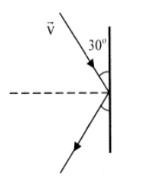
\includegraphics[width=0.2\linewidth]{../figs/VN12-Y24-PH-SYL-015P-1}
\end{center}
Xét 1 phân tử khí $\ce{H_2}$:
$$\Delta \vec{p}=\vec{f}\Delta t\Rightarrow 2mv\sin\alpha=p_1S\Delta t\Rightarrow p_1=\dfrac{2mv\sin\alpha}{S\Delta t}.$$
Áp suất do khí $\ce{H_2}$ tác dụng lên thành bình:
$$p=Np_1=\dfrac{2Nmv\sin\alpha}{S\Delta t}=\SI{3300}{\newton/\meter^2}.$$
}

\item \mkstar{3}\\
Một lượng khí thực hiện chu trình biến đổi trạng thái như hình bên. Cho biết: $t_1=\SI{27}{\celsius}$; $V_1=\SI{5}{\liter}$; $t_3=\SI{127}{\celsius}$; $V_3=\SI{6}{\liter}$. Ở điều kiện tiêu chuẩn, khí có thể tích $V_0=\SI{8.19}{\liter}$. Công do khí thực hiện sau một chu trình biến đổi trạng thái bằng bao nhiêu?
\begin{center}
	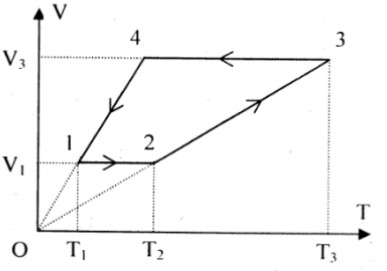
\includegraphics[width=0.35\linewidth]{../figs/VN12-Y24-PH-SYL-015P-4}
\end{center}
\hideall{
\begin{center}
	\begin{tabular}{|C{3cm}|C{3cm}|C{3cm}|C{3cm}|}
		\hline
		\thead{Trạng thái} & $p$ & $V$ & $T$\\
		\hline
		0 & $\SI{101325}{\pascal}$ & $\SI{8.19}{\liter}$ & $\SI{273}{\kelvin}$\\
		\hline
		 1 & $p_1$ & $\SI{5}{\liter}$ & $\SI{300}{\kelvin}$\\
		 \hline
		 2 & $p_2$ & $\SI{5}{\liter}$ & \\
		 \hline
		 3 & $p_2$ & $\SI{6}{\liter}$ & $\SI{400}{\kelvin}$\\
		 \hline
		 4 & $p_1$ & $\SI{6}{\liter}$ & \\
		 \hline
	\end{tabular}
\end{center}
$$\dfrac{pV}{T}=\text{const}\Rightarrow \dfrac{p_0V_0}{T_0}=\dfrac{p_2V_3}{T_3}\Rightarrow p_2=\SI{182385}{\pascal}.$$
Công do khí thực hiện trong chu trình là ở quá trình đẳng áp 2-3:
$$A_{23}=p_2\left(V_3-V_2\right)=\SI{182.385}{\joule}.$$
}

\end{enumerate}






